\chapter{Introduction}
\label{ch-introduction}
This work intends to contribute to Distribution Networks to improve power supply quality 
and reliability throughout Service Restoration (SR) methodologies. By reviewing and comparing 
the existing SR methodologies, it is possible to identify the challenges and the limitations 
of the current methodologies, in order to develop a solution that attempts to overcome them.
%Service Resotarion techniques by developing an algorithm that

In Chapter 1, the background and motivation of this work are presented. Additionally, and based on the 
identified challenges for SR improvements in distribution networks, the problem statement 
and research objectives are stated.  

\section{Background and Motivation}
\label{ch-introduction:sec:background}

Distribution Networks (DNs) allow supplying power to customers, and power quality and reliability ensure 
customer satisfaction. However, DNs are highly susceptible to failures, which causes more than 85$\%$ 
of power interruptions \cite{Liu2016}. That results not only in decreasing reliability indices but also in 
economic and social impacts \cite{Zidan2017}.

Therefore, there is a necessity to improve the DNs \cite{Kavousi-Fard2014}, whereby, in recent years, utilities 
invest in Distribution Automation (DA) intending to create a self-healing smart grid in order to improve 
SAIDI, SAIFI, and CAIDI indices \cite{Zidan2017}\cite{Angelo2013} \cite{Madani2015}. 
%maybe explain self-healing 

Distribution Automation (DA) takes advantage of available technologies to automate DN operations and enhance 
its performance \cite{U.S.DepartmentofEnergy2018}, since DNs became more difficult to 
design, manage, and sustain \cite{Madani2015}. Consequently, DA includes automated ways to locate the fault 
and restore the service in an optimized approach such as Fault Location, Isolation, and Service Restoration 
(FLISR) \cite{USDepartmentofEnergy2016} \cite{Liu2016}. 

FLISR operates after a fault detection. Firstly, it locates and isolates the fault as fast as possible. After 
the fault area is isolated, it transfers customers to healthy feeders and restores power supply to them 
\cite{Zidan2017}. Otherwise, customers may experience sustained outages \cite{USDepartmentofEnergy2016}. 

In a program conducted by the U.S. Department of Energy \cite{USDepartmentofEnergy2016}, it was shown that FLISR techniques achieve substantial 
DN operation improvements, such as a reduction in the number of customers interruptions (CI) by 55$\%$, and in 
customer minutes of interruption (CMI) by 53$\%$. \footnote{Average per event for FLISR operations reported by five utilities over one year \cite{USDepartmentofEnergy2016}.}

\begin{figure}
    \centering
	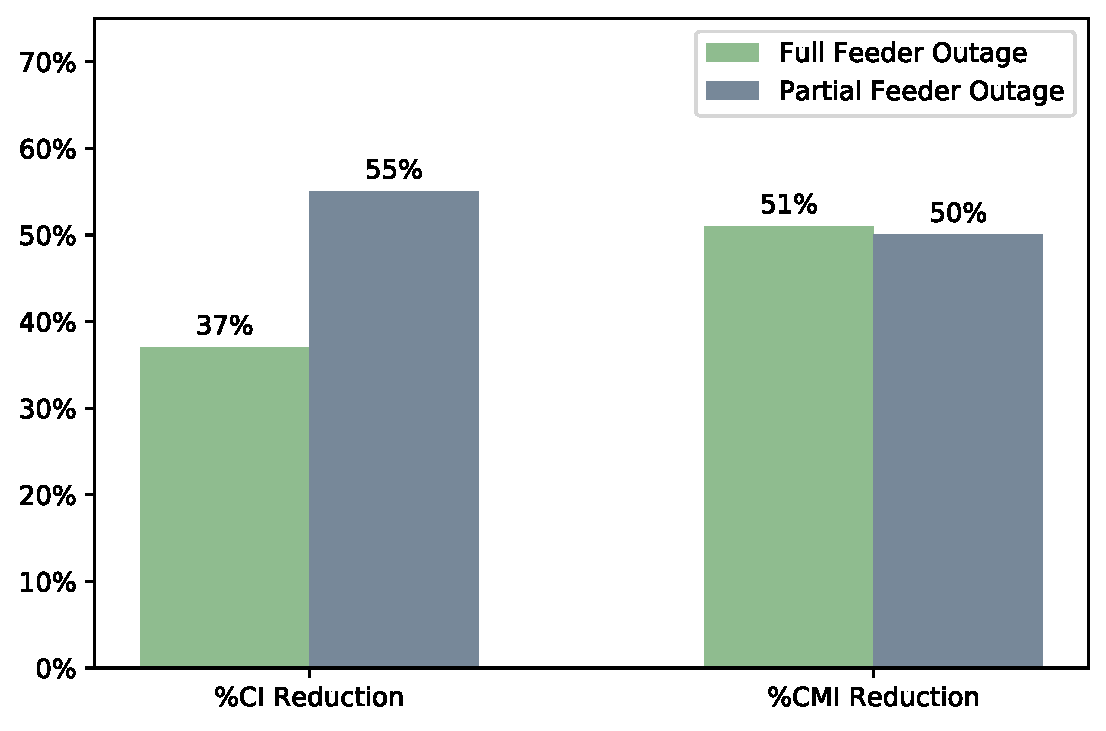
\includegraphics[scale = 0.5]{_introduction/fig/type_outage}
	\caption{FLISR effects on the number of customers interrupted (CI) and customer minutes of interruption (CMI) by the type of outage from USDON2016 \cite{USDepartmentofEnergy2016}.}
	\label{ch-introduction:fig:type_outage}
\end{figure}
\begin{figure}
    \centering
	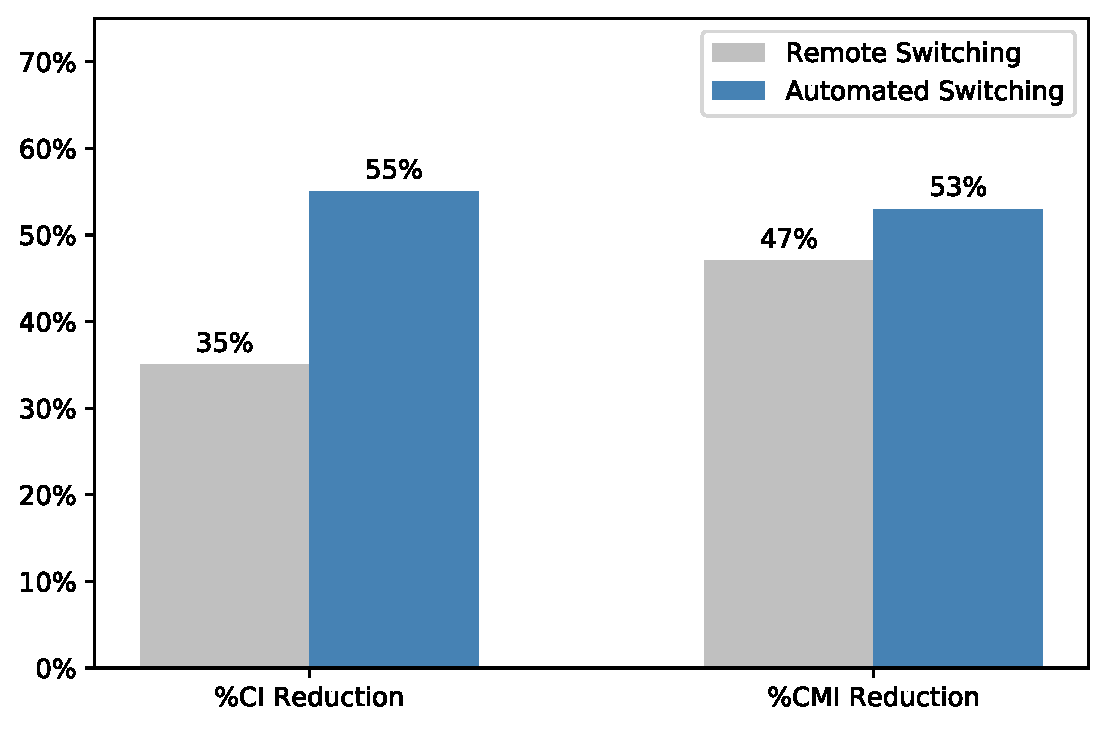
\includegraphics[scale = 0.5]{_introduction/fig/type_scheme.pdf}
	\caption{FLISR effects on the number of customers interrupted (CI) and customer minutes of interruption (CMI) by the type of FLISR operating scheme from USDON2016 \cite{USDepartmentofEnergy2016}.}
	\label{ch-introduction:fig:type_scheme}
\end{figure}

Figures \ref{ch-introduction:fig:type_outage} and \ref{ch-introduction:fig:type_scheme} show the reduction 
in CI and CMI by the type of outage and by type of FLISR scheme, respectively. The first figure states the 
number of customers interrupted decreases by 55$\%$ in a partial feeder outage, while the time of a full 
feeder outage decreases by 51$\%$. On the other hand, the second figure establishes that both CI and CMI 
have a further reduction when the FLISR scheme is automatic. Lastly, it should be pointed out these 
reductions improve directly the reliability indices mentioned before. 

As aforementioned, three stages constitute the FLISR scheme. The last stage is Service Restoration, one of the
most relevant strategies to enhance the resilience of DNs \cite{Shen2018}, and which is the main topic of this work.
%The problem is raised in the next section. 
\section{Problem Statement and Research Objectives}
\label{ch-introduction:sec:problem}

Service Restoration uses network reconfiguration methods to change the DN topology and resupply the out-of-service 
un-faulted customers \cite{Gholami2015}\cite{Shen2018}. This reconfiguration is carried out through 
switching operations, considering typical DNs have normally closed (NC) sectionalizing switches and normally 
opened (NO) tie switches \cite{Zidan2017} \cite{Sanches2014}. I.e., the main goal of SR is to find 
optimal switching sequences for the DN \cite{Latare2017}.

This procedure must maximize the number of loads restored, minimize the number of switching operations, and 
maintain operational and topological constraints \cite{Abu-Elanien2018} \cite{Gholami2015}. 
Nevertheless, and as noted in the formulation problem (Section \ref{ch-literature:sec:overview}), SR is computationally demanding because it is multi-objective, 
non-linear, and operational constrained. And also, it requires to explore a large number of switching operation 
combinations \cite{Shen2018} \cite{Sanches2014}. 

SR algorithm uses one or many techniques to obtain a solution, among which are expert systems, heuristic 
algorithms, meta-heuristic algorithms, graph theory, multi-agent systems, and mathematical programming \cite{Shen2018}. 
Furthermore, they can be implemented under centralized or decentralized approaches \cite{Zidan2017}. The control approaches 
and their corresponding techniques are reviewed, in further detail, in section \ref{ch-literature:sec:overview} and 
summarized in table \ref{ch-introduction:tab:sr_techniques}. 

\begin{table}
    \centering
    \caption{SR techniques comparison \cite{Abu-Elanien2018} \cite{Zidan2017}}
    \label{ch-introduction:tab:sr_techniques}
    \begin{tabular}{|l|c|c|c|}
        \hline
        \multicolumn{1}{|c|}{\textbf{Method}}                                        & \multicolumn{1}{c|}{\textbf{\begin{tabular}[c]{@{}c@{}}Optimal \\ solution\end{tabular}}} & \multicolumn{1}{c|}{\textbf{\begin{tabular}[c]{@{}c@{}}System \\ dependency\end{tabular}}} & \multicolumn{1}{c|}{\textbf{\begin{tabular}[c]{@{}c@{}}Self-learning \\ capacity\end{tabular}}} \\ \hline
        \textbf{Expert systems}                                                      & No                                                                                        & Yes                                                                                       & No                                                                                              \\ \hline
        \textbf{Heuristics}                                                          & No                                                                                        & Yes                                                                                       & No                                                                                              \\ \hline
        \textbf{Meta-heuristics}                                                     & No                                                                                        & Yes                                                                                       & No                                                                                              \\ \hline
        \textbf{\begin{tabular}[c]{@{}l@{}}Mathematical \\ programming\end{tabular}} & Yes                                                                                       & No                                                                                        & No                                                                                              \\ \hline
        \end{tabular}
\end{table}


Table \ref{ch-introduction:tab:sr_techniques} compares the different methodologies used to develop SR 
algorithms and shows their limitations. Most methodologies cannot obtain an optimal solution, 
but improvements in processing time \cite{Abu-Elanien2018}; thus, the solution optimality is sacrificed to obtain a faster solution. 
On the other hand, these methodologies, except mathematical programming, are system dependent and do not 
have the ability to self-learn, becoming out of date when system variations occur \cite{Zidan2017}.

Therefore, these limitations imply a need for human intervention to update their rules or knowledge bases 
and make the methodologies readapt to the new changes.

\subsection{General Purpose}

According to the previous data, the focus of this work is to develop a scalable Service Restoration algorithm 
capable of self-healing Distribution Networks by automatic learning the optimal sequence of switching 
operations to lead DNs to the best possible state after a fault occurs. Moreover, 
the challenge of automatic learning behavior also includes continuous learning, hence the system is 
constantly exploring to improve the sequence and adapt to changes in the network. Last but not least, 
the optimization objectives and constraints formalized in Chapter \ref{ch-literature} are also taken into account.

This work also aims to develop a validation system of the SR algorithm, which allows simulations of a 
practical distribution network and verification of its operational and topological constraints, 
through the integration of a co-simulation engine. 

\begin{enumerate}[
    labelindent=*,
    style=multiline,
    leftmargin=*,
    label=\textbf{Objective~\arabic*}]
        %\item Review existing methods for Service Restoration. 
        %\item Design a solution that improve the existing methods. 
        \item Develop a Service Restoration algorithm for Distribution Networks capable of self-learning to obtain an optimal solution that accomplishes operational and topological constraints by implementing a Reinforcement Learning technique.
        \item Develop a validation system that emulates and measures the parameters of a Distribution Network, in order to test the proposed SR algorithm performance, by integrating a co-simulation engine.
        %\item Develop a validation system by using co-simulation engine. 
\end{enumerate}
    




%This work intends to contribute to Service Resotarion techniques by developing an algorithm that improves the quality and reliability of distribution networks. By implementing Reinforcement Learning to create an agent capable of learning the best reconfiguration scheme feasible without violating DN constraints.As discussed in this thesis, Service Restoration. why is it important. However, successfully combining Machine Learning Techniques to reconfigure distribution networks is still an open research challenge.
